\chapter{Modelli lineari}

\section{Introduzione}
Alcuni approcci del machine learning fanno delle forti assunzioni riguardo i dati.
Questo avviene in quanto se le assunzioni sono vere si possono raggiungere performance migliori. 
Conoscenza pregressa del dominio ci permette di fare assunzioni sui dati.
In caso contrario l'approccio pu\`o fallire miseramente.
Altri approcci che non fanno molte assunzioni riguardo i dati invece permettono di imparare da dati pi\`u vari ma sono pi\`u proni a overfitting e richiedono pi\`u dati di training.

	\subsection{Bias}
	Il bias di un modello \`e quanto forte le assunzioni del modello sono.
	I classificatori a low-bias fanno delle assunzioni minime riguardo i dati come \emph{k-NN} (che assume unicamente che la vicinanza \`e correlata alla classe) e \emph{DT}, e quindi ci permettono di imparare sempre \emph{qualcosa}.
	I classificatori a high-bias fanno assunzioni forti riguardo ai dati.
	
\section{Linear separability}
L'assunzione strong-bias dei modelli lineari \`e la linear separability, ovvero che in due dimensioni le classi si possano separare attraverso una linea, mentre in dimensioni maggiori da un hyperplane.
Un modello lineare \`e pertanto un modello che assume che i dati sono linearmente separabili. 
	
	\subsection{Definire una linea}
	Ogni coppia di valori $(w_1,w_2)$ definisce una linea attraverso l'origine:
	$$0=w_1f_1+w_2f_2$$
	Si pu\`o inoltre vedere il vettore $\overrightarrow{w}=(w_1, w_2)$ come il vettore dei pesi perpendicolare alla linea.
	Per classificare i punti rispetto alla linea si considera il segno sostituendo i punti a $f_1$ e $f_2$.
	La positivit\`a o negativit\`a indica il lato della linea.
	Avere una linea che attraversa sempre l'origine è limitante, dunque i pu\`o estendere l'equazione con:
	$$a=w_1f_1+w_2f_2$$
	In questo modo la linea interseca l'asse delle $y$ in $a$. \ref{fig:chapter04-00}
	
	\begin{figure}
		\centering
		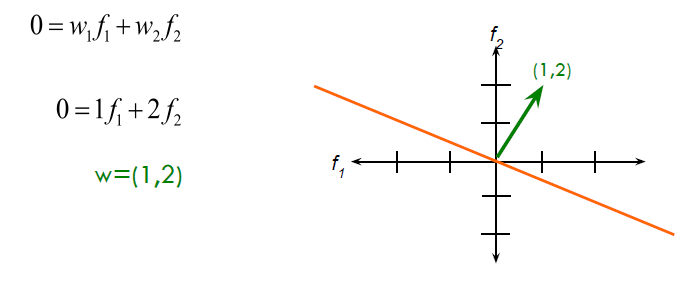
\includegraphics[width=0.6\linewidth]{imgs/chapter4/img0}
		\caption{Definire una linea}
		\label{fig:chapter04-00}
	\end{figure}

\section{Definizione di modello lineare}
Si definisce un modello lineare in uno spazio $n$ dimensionale, dove $n$ \`e il numero di features attraverso $n+1$ pesi.
$$0=b+\sum\limits_{i=1}^nw_if_i$$
In un modello lineare si classifica un nuovo esempio moltiplicandolo con il vettore dei pesi, aggiungendo il bias e controllando il segno del risultato.
Questo determina la classe dell'esempio. 
Siamo dunque interessati alla migliore coppia pesi e bias che separa i dati.

	\subsection{Training}
	Il training di un modello lineare avviene online, ovvero a differenza del modo in batch in cui vengono dati i training data come $\{(x_i, y_i):1\le i\le n\}$, i data points arrivano uno alla volta.
	L'algoritmo allora riceve un esempio $x_i$ senza label, predice la classificazione di questo esempio e confronta la predizione con la risposta corretta $y_i$.
	Infine aggiorna il proprio modello, dunque modifica la linea. 
	Se abbiamo tutti i dati a disposizione possiamo comunque fare training online.
	Le applicazioni del training online sono varie: data streams, dataset di grandi dimensioni, applicazioni che preservano la privacy.
	\subsection{Esempio di training}
	Supponiamo di avere il modello $w=(1,0)$ in figura \ref{fig:chapter04-02}. 
	Abbiamo appena ricevuto un punto in $(-1,1)$, le label ci dicono che quel punto dovrebbe essere classificato come positivo, ma al momento si trova nel lato negativo della linea. 
	Dunque i pesi vanno aggiornati.
	$$w_1*f_1 + w_2 * f_2 = 1 * -1 + 0 * -1 = -1$$
	
	Abbiamo ottenuto un risultato negativo, confermando che i pesi vadano aggiornati, al fine di ottenere un risultato positivo. 
	Possiamo scegliere vari modi per aggiornare i pesi, uno di questi \`e aggiornarli nel seguente modo: $w=(0,1)$, ottenendo il modello in figura \ref{fig:chapter04-03}.
	
	\begin{figure}
		\centering
		\begin{minipage}{.5\textwidth}
			\centering
			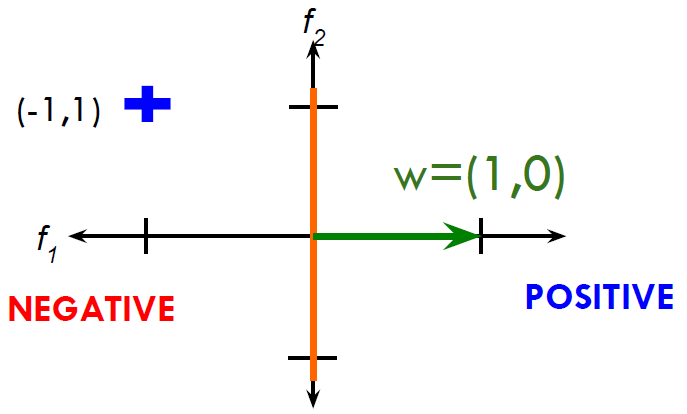
\includegraphics[width=1\linewidth]{imgs/chapter4/img2}
			\caption{Esempio: Modello}
			\label{fig:chapter04-02}
		\end{minipage}%
		\begin{minipage}{.5\textwidth}
			\centering
			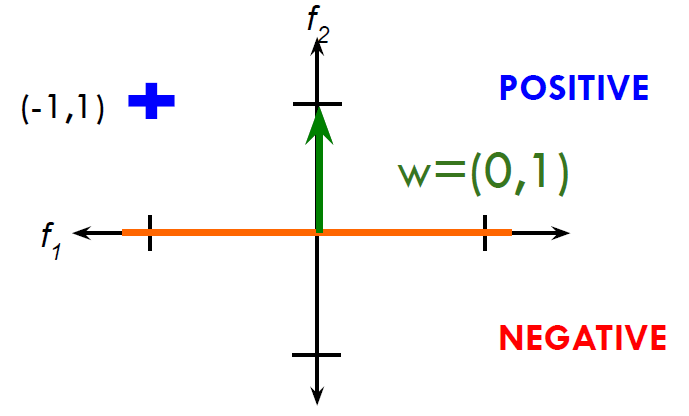
\includegraphics[width=1\linewidth]{imgs/chapter4/img3}
			\caption{Esempio: Modello aggiornato}
			\label{fig:chapter04-03}
		\end{minipage}
	\end{figure}
	
	\subsection{Perceptron}
	\`E un modello parametrico, \`e il blocco di base per la costruzioni di reti neurali.
		\subsubsection{Numero di iterazioni}
		Il numero di iterazioni del perceptron viene deciso in base alla convergenza.
		Inoltre pu\`o essere limitato in modo da ridurre l'overfitting.
		Si noti come in caso di dati non linearmente separabili la convergenza non avviene mai. 
		In caso di dati linearmente separabili abbiamo la garanzia di trovare \textbf{una} linea, non è detto che sia la migliore.
		
		\subsubsection{Ordine dei campioni}
		I campioni da considerare nel perceptron sono considerati in ordine casuale.
		In questo modo si produce un modello a low bias.
		
		\subsubsection{Linear separable sets}
		Le istanze di training sono linearmente separabili se esiste un hyperplane che separa le due classi. \ref{fig:chapter04-01}
		\begin{figure}
			\centering
			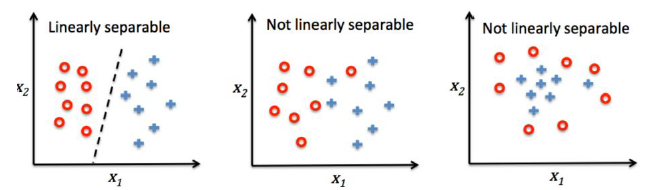
\includegraphics[width=0.6\linewidth]{imgs/chapter4/img1}
			\caption{Linear separable sets}
			\label{fig:chapter04-01}
		\end{figure}
		
		\subsubsection{Algoritmo}
		\input{Pseudocodice/01_perceptron}
		
		Meglio prendere esempi casuali, perch\`e l'ordine con cui prendiamo gli esempi influenza l'aggiornamento dei pesi.
		
		\subsubsection{Calcolo della predizione}
		\input{Pseudocodice/02_perceptron_prediction}

\section{Perceptron e reti neurali}
Si pu\`o immaginare il perceptron come un neurone artificiale o una funzione parametrizzata non lineare con un valore di attivazione soglia e un range di output ristretto.
Le reti neurali sono reti di neuroni artificiali densamente connessi in modo da simulare la rete di neuroni del cervello.

	\subsection{Funzione di attivazione}
	Una funzione di attivazione pu\`o essere una soglia dura: se la somma di tutti gli input \`e maggiore di un valore allora il perceptron manda il segnale queste permettono di imparare solo modelli lineari.
	Funzioni di attivazione pi\`u interessanti sono le sigmoidi, tangenti iperboliche, ReLU o rectified linear unit o leaky ReLU, perch\`e ci permettono di imparare modelli non lineari.
	
	\subsection{Storia del perceptron}
	Il perceptron nasce nel $1958$ da parte di Rosemblatt che lo crea con una soglia dura.
	Questo gli impedisce di imparare modelli non lineari come lo \emph{xor}.
	Viene superato nel $1986$ attraverso perceptrons multi layers e backpropagation e utilizzando una soglia meno dura.
